\chapter{Materials and Methods}

\section{Patients characterization}

This study is part of the research project entitled "Clinical utility of liquid biopsy in non-small cell lung cancer patients with EML4-ALK translocation". Its objective is to determine the best strategy for the identification of EML4-ALK translocations and to assess the clinical utility of periodic tumor monitoring in ALK-positive NSCLC patients from liquid biopsies. In this context, between June 2015 and July 2019, several ALK-positive NSCLC advanced subjects were recruited from 6 hospitals across Spain, including the Hospital Universitario Puerta de Hierro, the Complejo Hospitalario Universitario A Coruña, the Hospital Universitario Fundación Jiménez Díaz, the Hospital Clínic Barcelona, the Hospital General Universitario de Alicante, and the Hospital General Universitario de Valencia.

The primary study was conducted under the precepts of the Helsinki Declaration and was approved by the Hospital Puerta de Hierro Ethics Committee (internal code 79-18). Patients were eligible if they consented to allow their clinical information to be used in the previously mentioned research project. Their clinical history was queried for information on the age of diagnosis, sex, smoking status, histology, Eastern Cooperative Oncology Group (ECOG) status at the start of the study, stage, previous therapies, and date of death.

Eligible patients had histologically confirmed diagnosis of stage III–IV NSCLC that was ALK-positive, a measurable disease according to the response evaluation criteria in solid tumors (RECIST, version 1.1), were candidates to be treated with an ALK inhibitor, and were 18 years old or older. Exclusion criteria included the impossibility of frequent venipuncture or evidence of any other major clinical disorder or finding that would have made it undesirable for the patient to participate in the study.

\section{Laboratory Procedures}

To obtain the necessary data to develop the automatic algorithm for filtering genetic variants, a series of clinical procedures have been carried out, including the preparation and conditioning of the samples, their sequencing and analysis, and the subsequent confirmation of the ALK-positive samples.

\subsection{Sample Collection and Conditioning}

Once the EML4-ALK translocation has been diagnosed in a patient with NSCLC according to an anatomic pathology report (FISH and\slash or IHC), peripheral blood is extracted in a 9 $mL$ Streck Cell-Free DNA BCT\textsuperscript\textregistered{} (Streck, USA) tube and transported to the Liquid Biopsy Laboratory, where it is preserved until its conditioning.

In this study, isolation of cfDNA and exosomes from the cellular fraction was achieved by two consecutive centrifugation processes at room temperature, the first at 1500 $g$ for 10 $min$ and the second at 5000 $g$ for 20 $min$. After discarding the supernatant containing the clean plasma, cfDNA and exosome RNA isolation was performed using the QIAamp\textsuperscript\textregistered{} Circulating Nucleic Acid Kit (QIAgen, Valencia, CA, USA) and the exoRNeasy\textsuperscript\textregistered{} Serum/Plasma Maxi Kit (QIAgen, Valencia, CA, USA) respectively, following the manufacturer's instructions \cite{QUIAGEN_cfDNA, QUIAGEN_exosomes}. Until library preparation for sequencing, conditioned samples were stored at $-80$ \textdegree{C}.

Within the context of the project in which this thesis is included, blood samples have been extracted from patients in the pre-treatment stage, at months 2, 4, 6, 8, 12, 15 and 18, and at progression.

\subsection{Library Preparation}

Libraries were prepared from 10.4 $\mu L$ of cfDNA or exosome RNA using the Oncomine\texttrademark{} Pan-Cancer Cell-Free Assay (Thermo Fisher, Palo Alto, CA, USA) according to manufacturer's instructions \cite{Oncomine_PanCancer}. This multi-biomarker amplicon-based assay is optimized to detect more than 900 hotspots in 52 key genes from liquid biopsy samples containing tumor-derived DNA and RNA. It enables a limit of detection (LOD) down to 0.1\%, allowing the study of single nucleotide variants (SNVs), short insertions or deletions (indels), copy number variations (CNVs), and fusions. Specifically, the subsequent steps have been followed to prepare the NGS libraries (\autoref{fig:library}):

\begin{figure}[ht]
    \centering
    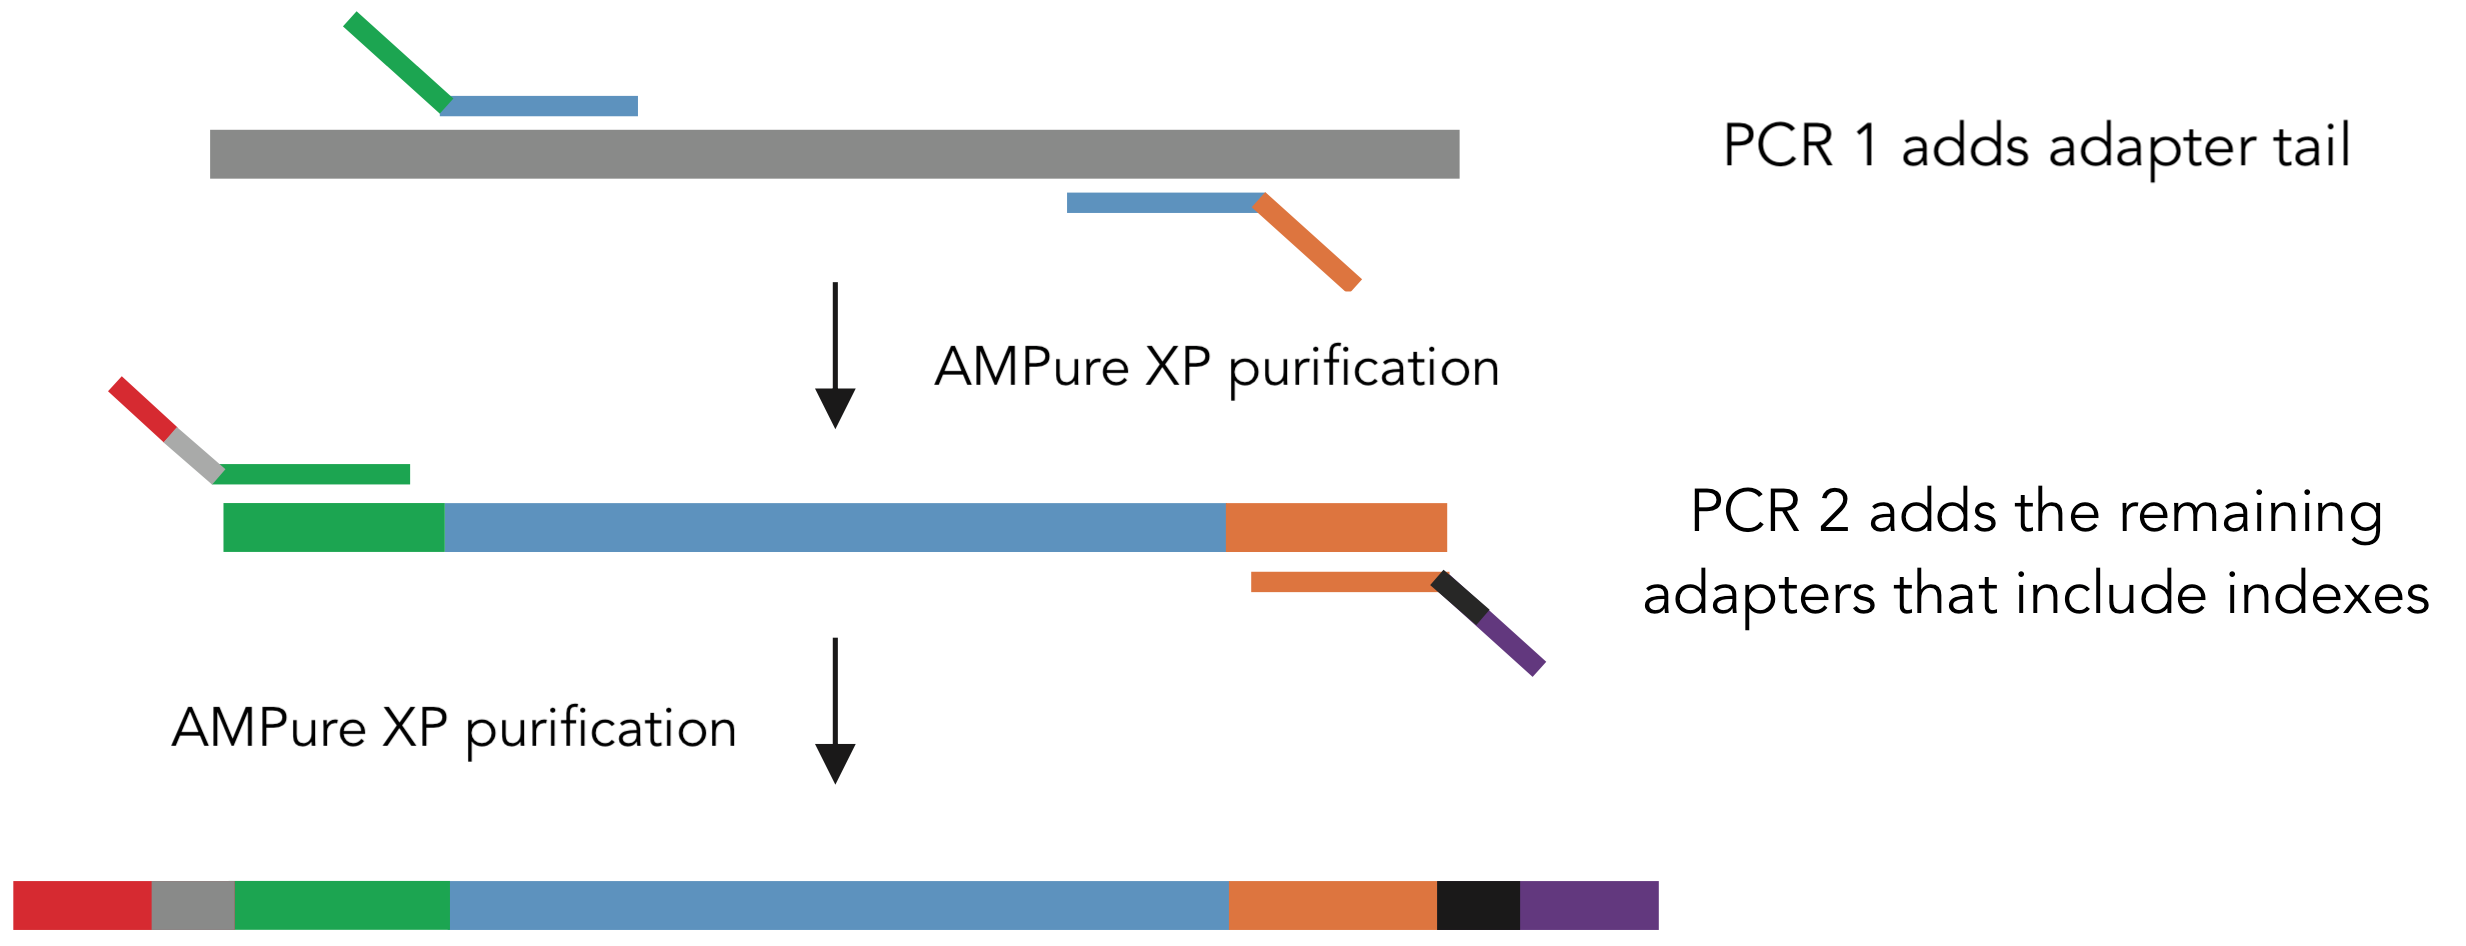
\includegraphics[width=0.85\textwidth]{Images/chapter_3/NGS_library.png}
    \caption{Amplicon-based library preparation.}
    \label{fig:library}
\end{figure}

\begin{enumerate}[font=\bfseries]
    \item \textbf{Reverse transcription of cell-free nucleic acids}. This step was only performed with exosome RNA samples, from which cDNA used for the following steps was synthesized.
    \item \textbf{Target amplification}. After the fragmentation of the isolated DNA using enzymatic methods, PCR amplification of these targets was used to produce labeled DNA amplicons within the desired size range.
    \item \textbf{Target amplicons purification}. Sample purification is a critical step for obtaining accurate NGS data. Therefore, in this study, a specific reagent with magnetic beads was used to remove short primers, unincorporated deoxyribonucleotide triphosphates (dNTPs), enzymes, short-failed PCR products, and salts from PCR fragments.
    \item \textbf{Amplification of the target amplicons with barcode adapted primers}. In this step, specific DNA adapter sequences were annealed to the 5' and 3' ends of the amplicon DNA. These adapters, among other functions, allow each sample to be marked with a specific nucleotide code, enabling the sequencer to analyze multiple patient samples simultaneously.
    \item \textbf{Barcoded library purification}. To guarantee reliable sequencing results, and in a process similar to the previous one, a purification of the labeled amplicons was carried out.
    \item \textbf{Size selection}. To isolate the DNA fragment sizes of interest for efficient and high-quality DNA sequencing, magnetic beads with varying concentrations of buffers were used in this step.
    \item \textbf{Library quantification}. To estimate the DNA concentration and to ensure equal representation of the indexed libraries, each of the samples was quantified with a qPCR and compared to the standard curve. Finally, the definitive barcoded libraries were pooled and adjusted to a final concentration of 50 $pM$.
\end{enumerate}

AMPure XP\textsuperscript\textregistered{} magnetic beads (Beckman Coulter, Inc., Brea, CA, USA) were used to carry out the purification and size selection steps \cite{AMPure}, while the Ion Library TaqMan\texttrademark{} Quantitation Kit (Thermo Fisher, Palo Alto, CA, USA) and the StepOnePlus\texttrademark{} Real-Time PCR System (Thermo Fisher, Palo Alto, CA, USA) were used for the quantification \cite{Quantification_TaqMan, qPCR_StepOnePlus}.

\subsection{Template Preparation}

%Ion Chef System Automates template preparation and Ion AmpliSeq library preparation

% ALK paper
%Eight samples were pooled.  Templating and Ion 550™ Chip loading were carried out on an Ion Chef™ System (Thermo Fisher, Palo Alto, CA, USA). Finally, an Ion GeneStudio™ S5 Sequencer (Thermo Fisher, Palo Alto, CA, USA) was used to sequence loaded Ion 550™ chips.

% MAT & MET
%Eight samples were pooled and templating and Ion 550™ Chip loading were carried out on an Ion Chef™ System (Thermo Fisher, Palo Alto, CA, USA). Finally, loaded Ion 550™ chips were sequenced on an Ion GeneStudio™ S5 Sequencer (Thermo Fisher, Palo Alto, CA, USA).

% CCLM
%Template preparation and chip loading were carried out on an Ion ChefTM System (Thermo Fisher, Palo Alto, CA, USA). Eight samples were loaded onto an Ion 530 Chip. Finally, loaded Ion 530TM chips were sequenced on an Ion S5TM Sequencer (Thermo Fisher, Palo Alto, CA, USA).


% TLCR
%Template preparation and chip loading were carried out on an Ion ChefTM System (Thermo Fisher, Palo Alto, CA, USA). Eight samples were loaded onto an Ion 550TM chip. Finally, Ion 550TM chips were sequenced in an Ion S5TM Sequencer (Thermo Fisher, Palo Alto, CA, USA).

\subsection{Sequencing}


\subsection{Data Analysis}

% MEMO 2007
% El análisis de los resultados de la dPCR será ciego a la información clínica del paciente. En cada tanda de PCR se incluirá un control negativo, otro positivo (DNA de líneas celulares portadoras de la translocación) y un blanco.

% ALK paper
% Torrent Suite Software (v5.10) was used to perform raw sequencing data analysis. The CoverageAnalysis (v. 5.10.0.1) plugin was used for sequencing coverage analysis (Thermo Fisher, Palo Alto, CA, USA). Raw reads were aligned to the human reference genome hg19. Variant calling, annotation and filtering were performed on the Ion Reporter (v5.10) platform using the Oncomine TagSeq Pan-Cancer Liquid Biopsy workflow (v2.1). Briefly, sequencing reads were mapped to defined target regions (Oncomine Pan-Cancer DNA Regions v1.0 (5.10)) and subjected to variant calling using Oncomine Pan-Cancer Annotations v1 r. 0. Integrative Genomics Viewer (IGV V.2.3.40, Broad Institute, Cambridge, MA, USA) was used to visualize sequencing reads.

% MAT & MET
% Analysis of raw sequencing data was performed using Torrent Suite Software (v5.10). For sequencing coverage analysis, the CoverageAnalysis (v. 5.10.0.1) plugin was used (Thermo Fisher, Palo Alto, CA, USA). Raw reads were aligned to the human reference genome hg19. Variant calling, annotation and filtering were performed on the Ion Reporter (v5.10) platform using the Oncomine TagSeq Pan-Cancer Liquid Biopsy w2.1. Briefly, sequencing reads were mapped to defined target regions (Oncomine Pan-Cancer DNA Regions v1.0 (5.10)) and subjected to variant calling using Oncomine Pan-Cancer Annotations v1 r. 0. For visualization of sequencing reads, the Integrative Genomics Viewer (IGV V.2.3.40, Broad Institute, Cambridge, MA, USA) was used.

%CCLM
% Analysis of raw sequencing data was performed using Torrent Suite Software (v5.6). For sequencing coverage analysis, the Coverag- eAnalysis (v. 5.6.0.1) plugin was used (Thermo Fisher, Palo Alto, CA, USA). Raw reads were aligned to the human reference genome hg19.
%Variant calling, annotation and filtering were performed on the Ion Reporter (v5.6) platform using the Oncomine Lung Liquid Biopsy workflow (v1.3), which is specifically designed to annotate low fre- quency (up to 0.1% limit of detection [LOD]) variants (SNPs, InDels) from targeted DNA libraries from the Oncomine Lung cfDNA Assay. Briefly, sequencing reads were mapped to defined target regions (Oncomine Lung cfDNA Regions v1.2 and Oncomine Lung cfDNA Hotspots v1.2) and subjected to variant calling using Oncomine Vari- ant Annotator v2.3 plugin. For visualization of sequencing reads, the Integrative Genomics Viewer (IGV V.2.3.40, Broad Institute, Cam- bridge, MA, USA) was used.

% TLCR
% The original EGFR-sensitizing mutation, and the p.T790M and p.C797S resistant mutations were analyzed by digital PCR (dPCR). Specifically, cfDNA was analyzed using commercially available predesigned TaqMan® Liquid Biopsy dPCR assays as well as custom TaqMan® assays in a QuantStudio® 3D Digital PCR System (Applied Biosystems, South San Francisco, CA, USA). dPCR reactions were carried out in a final volume of 18 μL and using 8.55 μL of cfDNA template. Subsequently, 14.5 μL were loaded into a QuantStudio 3D Digital PCR 20K chip. The cycling conditions were as follows: initial denaturation at 96 °C for 10 min, followed by 40 cycles at 56 °C for 2 min, and 98 °C for 30 s, a step of 72 °C for 10 min, and finally samples were maintained at 22 °C for at least 30 min. Chip fluorescence was measured twice. Results were analyzed with QuantStudio® 3D AnalysisSuiteTM Cloud Software. The automatic call assignments for each data cluster were manually adjusted when needed. The result of the assay is reported as the ratio of mutant DNA molecules relative to the sum of mutant and wild-type (wt) DNA molecules. A negative and a positive control DNA were included in every run.

\subsection{Confirmation of the Sequenced Results}

% ALK paper
% The mutations identified by NGS were confirmed by digital PCR (dPCR) on cfDNA samples using a QuantStudio® 3D Digital PCR System (Applied Biosystems, South San Francisco, CA, USA). As per manufacturer's specifications, dPCR reactions were performed in 18 μL volumes using 9 μL of 20X QuantStudio 3D Master Mix, 0.45 μL of 40X commercially available predesigned or custom TaqMan® assays and 8.55 μL of cfDNA. 14.5 μL of the reaction volume were loaded onto a QuantStudio 3D Digital PCR 20K chip using QuantStudio™ 3D Digital PCR Chip Loader. Each dPCR run included a negative control DNA, as a wild-type (wt) control, and a white. PCR reaction was performed in a thermal cycler (Applied Biosystems) at 96 °C for 10 min, then 40 cycles at 56 °C for 2 min and 98 °C for 30 s, and a final elongation step 72 °C for 10 min. Finally samples were maintained at 22 °C for at least 30 min. After dPCR was completed, chips were loaded into two QuantStudio™ 3D Digital PCR Instruments to reads the fluorescence twice. The readers used an image capture to perform a preliminary analysis and subsequently, data were visualized and analyzed using QuantStudio® 3D Analysis Suite™ Cloud Software. Briefly, the automatic call assignments for each data cluster were manually adjusted when needed. The target concentration was calculated as the ratio of mutant DNA molecules relative to the sum of mutant and wild-type (wt) DNA molecules. Samples with a mutant allele fraction (MAF) equal to or higher than 0.1% were considered positive. The LOD was assessed for all individual assays, being lower than 0.1% in all cases.

% MAT & MET
% Mutation confirmation was performed by digital PCR using cfDNA or cDNA. The reverse transcription of platelets and exosomes RNA were performed using PrimeScript™ RT Reagent Kit (TaKaRa, Japan) according to the manufacturer's instructions. To aim, cfDNA or cDNA samples were analyzed using commercially available predesigned TaqMan® Liquid Biopsy dPCR assays and custom TaqMan® assays on a QuantStudio® 3D Digital PCR System (Applied Biosystems, South San Francisco, CA, USA). For the dPCR reaction, 9 μL of 20 × QuantStudio 3D Master Mix was mixed with 0.45 μL of the aforementioned 40X TaqMan® assays and 8.55 μL of template DNA 14.5 μL of the reaction volume were loaded onto a QuantStudio 3D Digital PCR 20K chip using QuantStudio™ 3D Digital PCR Chip Loader. The thermal cycler method was as follows: initial denaturation at 96 °C for 10 min, followed by 40 cycles at 56 °C for 2 min and 98 °C for 30 s and an elongation step of 72 °C for 10 min, and finally samples were maintained at 22 °C for at least 30 min. when cycling was complete, chip fluorescence was read twice using two QuantStudio™ 3D Digital PCR Instruments, which performs a preliminary analysis using an image capture. Results were analyzed using QuantStudio® 3D Analysis Suite™ Cloud Software. The automatic call assignments for each data cluster were manually adjusted when needed. The result of the assay was reported as the ratio of mutant DNA molecules relative to the sum of mutant and wild-type (wt) DNA molecules. A negative control DNA and a white were included in every run. Samples were considered positive when the mutant allele fraction (MAF) was greater than or equal to 0.1%. The LOD was assessed for all individual assays, being less than 0.1% in all cases.

% CCLM
%Mutations with a minor allele frequency equal to or higher than 0.1%, detected in at least two molecular counts, were consid- ered positive. Mutation confirmation was performed by dPCR. To this aim, cfDNA samples were analyzed using commercially avail- able predesigned TaqMan® Liquid Biopsy dPCR assays and custom TaqMan® assays on a QuantStudio® 3D Digital PCR System (Applied Biosystems, South San Francisco, CA, USA) to confirm the previ- ously detected mutations. For the dPCR reaction, 8.55 μL of template cfDNA was mixed with 0.45 μL of the aforementioned 40X TaqMan® assays and 9 μL of 20 ×  QuantStudio 3D Master Mix, in an 18-μL reaction volume. As previously reported [6], 14.5 μL were loaded into QuantStudio 3D Digital PCR 20K chips. The cycling conditions were as follows: initial denaturation at 96 °C for 10 min, followed by 40 cycles at 56 °C for 2 min and 98 °C for 30 s and an elongation step of 72 °C for 10 min, and finally samples were maintained at 22 °C for at least 30 min. Chip fluorescence was read twice. Results were analyzed using QuantStudio® 3D Analysis SuiteTM Cloud Software. The automatic call assignments for each data cluster were manually adjusted when needed. The result of the assay is reported as the ratio of mutant DNA molecules relative to the sum of mutant and wild-type (wt) DNA molecules. A negative control DNA was included in every run. Samples were considered positive when the mutant allele frac- tion (MAF) was greater than or equal to 0.1%. The LOD was assessed for all individual assays as previously described [4, 7]. In all cases, the LOD was below 0.1%.

% TLCR
% Raw sequencing data were analyzed using Torrent Suite Software (v5.10.0). Sequencing coverage was analyzed using the Coverage Analysis (v.5.10.0.3) plug-in (Thermo Fisher, Palo Alto, CA, USA). Raw reads were aligned to the human reference genome hg19.
% Variant calling, annotation and filtering were carried out on the Ion Reporter (v5.10) platform using the Oncomine TaqSeq Pan-Cancer Liquid Biopsy workflow (v5.10). The clinical significance of somatic variants was determined according to the Standards and Guidelines for the Interpretation and Reporting of Sequence Variants in Cancer (14). Mutations with an allele frequency (AF) greater than or equal to 0.1% were considered positive.

\subsection{Algorithm development}



